\documentclass[12]{amsart}

\usepackage{amssymb,amsmath}

%\usepackage{refcheck}

\usepackage{graphicx}
\usepackage{amssymb}
\usepackage{mathrsfs}
\usepackage{amsmath}
\usepackage{latexsym}
\usepackage{amssymb}
\usepackage{enumerate}
\usepackage{fullpage} 
\usepackage{setspace}
\usepackage{color}
%\usepackage{ dsfont }
\usepackage{float}
\usepackage{physics}

%new math symbols taking no arguments
\newcommand\0{\mathbf{0}}
\newcommand\CC{\mathbb{C}}
\newcommand\FF{\mathbb{F}}
\newcommand\NN{\mathbb{N}}
\newcommand\QQ{\mathbb{Q}}
\newcommand\RR{\mathbb{R}}
\newcommand\ZZ{\mathbb{Z}}
\newcommand\bb{\mathbf{b}}
\newcommand\kk{\Bbbk}
\newcommand\mm{\mathfrak{m}}
\newcommand\pp{\mathfrak{p}}
\newcommand\xx{\mathbf{x}}
\newcommand\yy{\mathbf{y}}
\newcommand\GL{\mathit{GL}}
\newcommand\into{\hookrightarrow}
\newcommand\nsub{\trianglelefteq}
\newcommand\onto{\twoheadrightarrow}
\newcommand\minus{\smallsetminus}
\newcommand\goesto{\rightsquigarrow}
\newcommand\nsubneq{\vartriangleleft}

%redefined math symbols taking no arguments
\newcommand\<{\langle}
\renewcommand\>{\rangle}
\renewcommand\iff{\Leftrightarrow}
\renewcommand\phi{\varphi}
\renewcommand\implies{\Rightarrow}

%new math symbols taking arguments
\newcommand\ol[1]{{\overline{#1}}}

%redefined math symbols taking arguments
\renewcommand\mod[1]{\ (\mathrm{mod}\ #1)}

%roman font math operators
\DeclareMathOperator\aut{Aut}

%for easy 2 x 2 matrices
\newcommand\twobytwo[1]{\left[\begin{array}{@{}cc@{}}#1\end{array}\right]}

%for easy column vectors of size 2
\newcommand\tworow[1]{\left[\begin{array}{@{}c@{}}#1\end{array}\right]}

\newtheorem{theorem}{Theorem}[section]
\newtheorem{corollary}{Corollary}[theorem]
\newtheorem{lemma}[theorem]{Lemma}
\newtheorem{exercise}[theorem]{Exercise}

\doublespacing
\title[PHY 493 Final Paper]{A Review of Quantum Machine Learning}
\author{Faris Sbahi}
\begin{document}
\maketitle

\section{Introduction}

Machine learning explores the study and construction of algorithms that are capable of finding patterns in data. Hence, this entails studying the ability of learning models to capture these patterns and generalize, as one would in statistical learning theory, in addition to studying model efficiency, enabled by computational complexity theory. In practice, many of the widely used supervised and unsupervised machine learning models can reasonably be described as linear algebraic data analysis techniques. For example, consider that ordinary least squares regression and ridge regression can be given in terms of a closed-form product of matrices and matrix inverses and that principal component analysis is essentially solving for the largest-eigenvalue eigenvectors of a particular covariance matrix. Furthermore, optimization problems, which are common in machine learning, can often be broken down into a set of basic linear algebraic subproblems.

Since its conception, quantum computation and quantum information has taught us to "think physically about computation" \cite{nielsen2010quantum}. Well, if quantum mechanics tells us that physical states are mathematically linear algebraic objects (vectors in a Hilbert space), then perhaps this lesson says that the type of computation best suited for quantum physical reality are linear algebraic problems, such as the machine learning ones noted above. This somewhat naive intuition turns out to have value, as we will show in this review.

Hence, this leads us to the idea of quantum machine learning which uses quantum algorithms as part of a larger implementation to outperform the corresponding classical learning algorithms.

Nevertheless, past linear algebraic analysis techniques, there exist other classes of machine learning algorithms such as deep learning built on artificial neural networks and reinforcement learning which models an environment as a Markov decision process \cite{sutton1998reinforcement}. Successes have been achieved in terms of quantum speedups in these arenas \cite{dong2008quantum}, but we won't explore these alternative machine learning routes further in our review. 

In this review, we will cover the main theoretical results in terms of quantum algorithms relevant to quantum machine learning. Then, we'll describe specific learning problems that have achieved quantum speedups using these results. Finally, we'll discuss important limitations to these results which may pose substantive challenges to the future of quantum learning theory.

Our goal is to provide a birds-eye view of these concepts and refer the reader to appropriate references where they desire greater detail. We assume that the reader is familiar with the fundamentals of quantum information theory e.g. by means of Chapter 2 of \cite{nielsen2010quantum}.

\section{Comparing Machine Learning Performance}

If we are to claim that some machine learning algorithms perform better on a quantum computer, we first must decide on a notion of "outperforming". 

This is currently characterized by the advantage in runtime obtained by a quantum algorithm over the classical methods for the same task. We quantify the runtime with the asymptotic scaling of the number of elementary operations used by the algorithm with respect to the size of the input, as one does in complexity theory. 

The definition of an elementary operation is dependent on the choice of measure of complexity. Query complexity measures the number of queries to the information source for the classical or quantum algorithm. Hence, a quantum speedup results if the number of queries needed to solve a problem is lower for the quantum than for the classical algorithm \cite{biamonte2017quantum}.

\section{Speedup Techniques}

\subsection{Grover's Algorithm and Amplitude Amplification}

Suppose we wish to search a space of elements of size $N$. Clearly this problem is $\Omega(N)$, classically. Rather than searching the elements directly, we can focus on "searching" their indices which are labelled $[ 0, N-1]$ by using an oracle. So, let $x \in [0, N-1]$ and $\ket{q}$ be an ancillary qubit. Define $f(x) = 1$ if the index is the index of the solution and $f(x) = 0$ otherwise. An oracle is a unitary operation, $O$, which acts on the computation basis as

\begin{align*}
\ket{x}\ket{q} \rightarrow^O \ket{x}\ket{q \oplus f(x)}
\end{align*}

Hence, if we let $\ket{q} = \frac{\ket{0}-\ket{1}}{\sqrt{2}} = \ket{-}$, then we can rewrite this transformation as

\begin{align*}
\ket{x}\ket{-} \rightarrow^O (-1)^{f(x)}\ket{x}\ket{-}	
\end{align*}

Grover \cite{grover1996fast} came up with a quantum algorithm that finds a solution with high probability using $O(\sqrt{N})$ oracle queries (which is known to be optimal on a quantum computer \cite{nielsen2010quantum}).

For $N = 2^n$, the grover iteration can be given by the linear transformation $G = (2\ket{\psi}\bra{\psi}-I)O$ where $\ket{\psi}$ is the equally weighted superposition of states. 

So, assuming that the number of solutions $M = 1$, Grover's algorithm essentially prepares $N$ qubits in state $\ket{\psi}\ket{-}$ and then applies $G$ for $\frac{\pi}{4}\sqrt{N}$ iterations. 

However, if the number of solutions $M \geq 1$ is unknown, then a variant, known as amplitude amplification \cite{brassard2002quantum}, can be used to find a solution in the solution subspace with high probability using $O(\sqrt{N/M})$ queries. 
   
\subsection{Solving Systems of Linear Equations}

Solving linear systems of equations is a ubiquitous problem in machine learning. As we will discuss, many learning problems, such as least-squares regression and least-squares SVMs, require the inversion of a matrix. Hence, we will describe two common quantum algorithms which lead up to the recent HHL algorithm, named after the algorithm's authors, Harrow, Hassidim, and LLoyd.

\subsubsection{Quantum Fourier Transform}

In the following, we take $N = 2^n$, where $n$ is some integer. Hence, the quantum Fourier transform on the orthonormal computational basis $\{ \ket{0}, \cdots ,\ket{N - 1} \}$ for an $n$ qubit quantum computer is defined to be a linear operator with the following action on the basis states,

\begin{align*}
\ket{j} \rightarrow \frac{1}{\sqrt{N}} \sum_{k=0}^{N-1} e^{2\pi i jk / N} \ket{k}	
\end{align*}

The gate complexity on a quantum computer is $O(n^2)$ as opposed to $O(n2^n)$, classically, using the technique in \cite{nielsen2010quantum}. Hence, at first glance, the potential quantum speedup via this subroutine is phenomenal for many machine learning and data analysis tasks. For example, speech recognition preprocessing begins with a Fourier transform of the digitized sound. 

However, there is no way of determining the Fourier transformed amplitudes of the original state. Hence, the applications are more subtle than one may have expected.

\subsubsection{Phase Estimation}

Suppose a unitary operator $U$ has an eigenvector $\ket{u}$ with eigenvalue $e^{2\pi i \phi}$, where the value of $\phi$ is unknown. 

The phase estimation algorithm uses two registers: one of $t$ qubits in the equal superposition state and another which stores $\ket{u}$. Then, after a series of controlled-$U^{2^j}$ operations on the $j$th qubit and an inverse Fourier transform, the first register holds the state $\ket{\phi_1 \cdots \phi_t}$, which is an approximation of $\phi$, whose accuracy is dependent on the size of $t$. 

Hence, the complexity of this algorithm is essentially that of the inverse Fourier transform, $O(t^2)$. This assumes that each controlled-$U^{2^j}$ operation is given by an oracle, which may not hold in practice. Furthermore, we also assume that we can prepare $\ket{u}$ efficiently, which also may not hold in practice. Hence, we often require workarounds to these problems in our applications of Phase Estimation.

\subsubsection{HHL Algorithm}

One such application of Phase Estimation is with respect to solving linear systems of equations. This is the so-called HHL algorithm \cite{lloyd2010quantum}. Here, we will cover the essential details of the algorithm.

The general problem statement of a linear system is if we are given matrix $A$ and unit vector $\vec{b}$, then find $\vec{x}$ satisfying, 

$$A\vec{x} = \vec{b}$$ 

However, assume that instead of solving for $x$ itself, we instead solve for an expectation value $x^T M x$ for some linear operator $M$. The original description of the algorithm provides runtime bound of $\tilde{O}(\log(N)\kappa ^{2} s^2 / \epsilon)$, where $s$ is sparsity measured by the maximum number of non-zero elements in a row and column of $A$, $\kappa$ is the condition number, and $\epsilon$ is the approximation precision. Hence, we can only achieve speedup if the linear system is sparse and has a low condition number $\kappa$. Ambainis \cite{ambainis2012variable} and Childs \cite{childs2015quantum} improved this depency on $\kappa$ and $s$ to linear and $\epsilon$ to poly-logarithmic.

This compares well considering that the best classical algorithm has a runtime of $O(N^{2.373})$ \cite{coppersmith1987matrix}. However, due to the large amount of pre-processing required, the algorithm is not used in practice. Standard methods, for example, based on QR-factorization take $O(N^3)$ steps \cite{golub2012matrix}. 

So, assume that $A$ in our linear system is an $N \times N$ Hermitian matrix. Notice that this is an "unrestrictive" constraint on $A$ because we can always take non-Hermitian matrix $A'$ and linear system $A' \vec{x} = \vec{b}$ and instead solve $\begin{bmatrix}
	0 && A' \\ A'^\dag && 0
\end{bmatrix} \begin{bmatrix} 0 \\ x \end{bmatrix} = \begin{bmatrix} b \\ 0 \end{bmatrix}$. Hence, we we will assume that $A$ is Hermitian from here on. 

Recall that because $A$ is hermitian, then we can perform quantum phase estimation using $e^{-iAt}$ as the unitary transformation. This can be done efficiently if $A$ is sparse.

So, we first prepare $\ket{b} = \sum_i b_i \ket{i}$ (the representation of $\vec{b}$). We assume that this can be done efficiently or that $\ket{b}$ is supplied as an input.

Denote by $\ket{\psi_j}$ the eigenvectors of $A$ with associated eigenvalues $\lambda_j$. Hence, we can express $\ket{b}$ as $\ket{b} = \sum_j \beta_j \ket{\psi_j}$.  So, we initialize a first register to state $\sum_j \beta_j \ket{\psi_j}$ and second register to state $\ket{0}$ . After applying phase estimation, we then have the joint state $\sum_j \beta_j \ket{\psi_j} \ket{\widetilde{\lambda}_j}$, where $\widetilde{\lambda}_j$ is an approximation of $\lambda_j$. We'll assume that this approximation is perfect from here on, for the sake of demonstration. 

Next we add an ancilla qubit and perform a rotation conditional on the first register which now holds $\ket{\lambda_j}$. The rotation transforms the system to

\begin{align*}
\sum_j \beta_j \ket{\psi_j} \ket{\lambda_j} \Big(\sqrt{1-\frac{C^2}{\lambda_j^2}}\ket{0} + \frac{C}{\lambda_j}\ket{1}\Big)
\end{align*}

for some small constant $C \in \RR$ that is $O(1/\kappa)$.

Hence, we can undo phase estimation to restore the second register to $\ket{0}$.

One sees that if we measure the ancillary qubit in the computational basis, we'll evidently collapse the state to $\ket{1}$ with probability $\Omega(1/\kappa^2)$. However, using amplitude amplification this can be upper-bounded to $O(1/\kappa)$.  

Finally, we can make a measurement $M$ whose expectation value $\bra{x}M\ket{x}$ corresponds to the feature of $x$ we wish to evaluate. 

The concessions we noted along the way clearly limit the algorithm's applicability to practical problems. We have three essential caveats to achieving exponential speedup: (1) $A$ must be sparse and have a condition number that scales at most sublinearly with $N$, (2) $\ket{b}$ must be loaded in quantum superposition in $\log(N)$ time, and (3) $\ket{x}$ isn't actually be read out, but instead an expectation is computed.


Limitation (1) has been partially resolved by the work of \cite{wossnig2018quantum} to achieve a quadratic speedup for dense matrices. 

Limitation (2) may be solved by quantum RAM, which then has its own limitations discussed in the next section. 

Limitation (3) is a general issue with regards to reading out classical information from a quantum state at the conclusion of a quantum algorithm because we would need at least $N$ measurements to retrieve this classical data. Hence, this would eliminate the potential for exponential speed-up.  

Hence, after observing these limitations we may wonder if there can exist a classical algorithm with the same caveats that can achieve the same runtime. Importantly, in the original paper the authors showed that HHL is “universal for quantum computation.” Hence, we can encode any quantum algorithm e.g. Shor's algorithm into a system of roughly $2^n$ linear equations in $2^n$ unknowns, and then use HHL to “solve” the system (i.e., simulate the algorithm) in polynomial time. Thus, provided we believe any quantum algorithm achieves an exponential speedup over the best possible classical algorithm, HHL can in principle achieve such a speedup as well.

To conclude, HHL is a logarithmic time quantum algorithm for matrix inversion, a task arising in many learning problems. However, a number of caveats that include the requirement of a logarithmic access time to the memory and the impossibility of retrieving the solution vector with one measurement lead to the question of whether classical or parallel algorithms that make use of the same assumptions obtain similar, or better, runtimes in practice. Hence, we will need empirical data to further address this question.

\subsection{Quantum Random Access Memory} 

The essence of machine learning is analyzing a vast amount of data. Hence, we must address the question of how classical data is encoded in quantum superposition, a concern brought up in our previous discussion of the matrix inversion algorithm. 

So, assume that we have an classical vectors $\{v_1, \cdots , v_ n : v_1 \in \RR^m \}$ that need to be encoded for use as part of a quantum algorithm. Quantum random access memory (qRAM) can encode these classical vectors in superposition into $\log(nm)$ qubits in $\log(nm)$ time using its "bucket-brigade architecture"\cite{giovannetti2008quantum}. The basic idea is to use a three-level tree structure where the $nm$ qubit "leaves" contain the entries of the $n$ vectors in $\RR^m$.

One of the central limitations of qRAM is that the number of resources scales as $O(nm)$ i.e. exponentially in the binary representation of $n, m$. There have been open questions of the viability of this model of memory, in practice. In particular, if each of the qubits must be error-corrected, then it seems entirely impractical for general use. Some of this concern has been answered by proponents who have showed that, given a certain error model, algorithms that require to query the memory a polynomial number of times (e.g. the HLL algorithm above) might not require fault-tolerant components. Still, the amplitude amplification algorithm above does require this error correction. 

Furthermore, it may be only fair to compare qRAM to a parallel classical architecture, given that we are allowing resources to scale exponentially. 

Considerable, too, is the fact that data must be distribute fairly uniformly over the quantum register or else qRAM is no longer efficient \cite{aaronson2015read}. 

In conclusion, qRAM comes with a significant number of considerations in itself and hence should be subjected to empirical investigation to determine its genuine quantum speed-up in practice. 

%\section{Inner Product Evaluation}

\section{Applications}

\subsection{Principal Component Analysis}

First, we consider the ubiquitous principal component analysis (PCA) algorithm. PCA reduces the dimensionality of data by transforming the features to uncorrelated weightings of the original features ("principal components"). This requires simply finding the eigenvalues and eigenvectors of the data covariance matrix. 

Hence, let $v_j \in V$ where $V$ is a $d$-dimensional vector space such that $d=2^n=N$ and assume that $|v_j| = 1$ for simplicity. Hence, the covariance matrix of the data is given by $C = \sum_j v_jv_j^T$ whose eigenvalues and eigenvectors we seek to discover. So, suppose we can prepare quantum state $v_j \rightarrow \ket{v_j}$, choosing classical data vector $v_j$ uniformly at random. For example, we can use qRAM, discussed above. Then, because of our random selection, the resulting quantum state has density matrix $\rho = \frac{1}{N} \sum_j \ket{v_j}\bra{v_j}$ which we observe to be the covariance matrix, up to an overall factor. 

Then, as Lloyd, Mohseni and Rebentrost describe \cite{lloyd2014quantum}, one way to perform quantum PCA use that given $n$ copies of $\rho$ we have the ability to apply the unitary operator $e^{-i\rho t}$ to any state $\sigma$ with accuracy $O(t^2 / n)$. This can be done by using repeated infinitesmal applications of the SWAP operator on $\rho \otimes \sigma$. 

Hence, using $e^{-i \rho t}$, we can perform phase estimation on $rho$. So, let $\ket{\psi_i}$ be the eigenvectors of $\rho$ with associated eigenvalues $\lambda_i$ and so $\rho = \sum_j \lambda_j \ket{\psi_j}\bra{\psi_j}$. Therefore, phase estimation gives u

\begin{align*}
\sum_j \lambda_j \ket{\psi_j}\bra{\psi_j} \otimes \ket{\tilde{\lambda_j}} \bra{\tilde{\lambda_j}}
\end{align*}

where $\tilde{\lambda_j}$ is an approximation of $\lambda_j$. Hence, if we measure the second register and repeat this procedure several times, the most frequent outcome is the first principal component $\ket{\psi_{max}}$, and so on.

The algorithm works best when a small number of principal components have significantly greater eigenvalues than the rest. Hence, $\rho$ is well represented by the subspace spanned by the principal components. In particular, let $m << d$ be the dimension of the subspace of principal components which represent $\rho$ within some bound. Then, the algorithm has runtime $O(m \log n )$. 

Hence, this gives a limitation: if the eigenvalues of the covariance are roughly equal and of size $O(1/d)$, then the algorithm reduces to scaling in time $O(d)$ (as does the classical algorithm). Furthermore, we evidently inherit the limitations of qRAM, if we use it for the state preparation above.  

\subsection{Support Vector Machines}

Support vector machines seek to find an optimal (maximum margin) separating hyperplane between two classes of data in a dataset. Hence, if the training data is linearly separable, each class can be found on only one side of the hyperplane. In particular, let $\{ x_1 , \cdots , x_n \}$ be a set of observations where $x_i$ is a $d$-dimensional vector with associated labels $y_i \in \{ 0 , 1\}$. Hence, we seek a linear function $f(x) = \vec{w} \cdot \vec{x} - \vec{b}$ where $\vec{w}$ is a weight vector and $\vec{b}$ is a bias vector s.t. $y_if(x_i) > 0, \forall i$. Furthermore, we seek to maximize the minimum $y_i f(x_i)$, across all $i$. 

\begin{figure}[H]
\centering
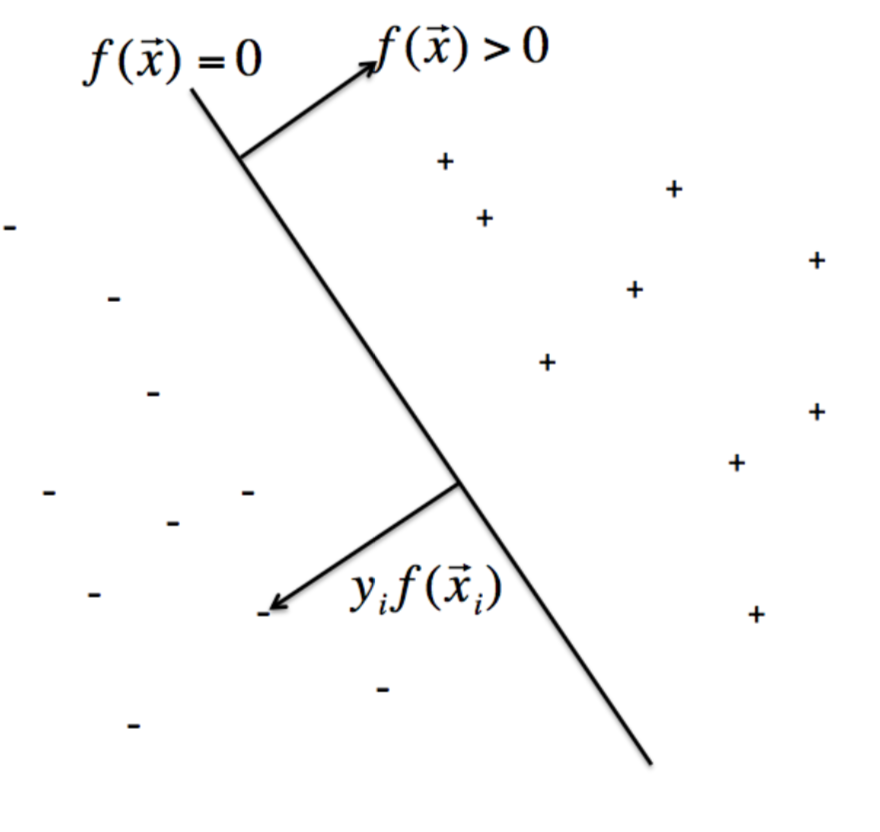
\includegraphics[width=0.5\linewidth]{svm.png}	
\caption{Visualization of a separating hyperplane and its associated margin taken from \cite{rudin}.}
\end{figure}

Much of the appeal of SVM is in its generalization to nonlinear hypersurfaces by replacing the constituent inner products with a kernel that implicitly maps the observations to another high dimensional space \cite{rudin}.% This mapping can be represented by a kernel ma

Solving SVM generally is performed by optimization of the dual problem which is a quadratic optimization problem. Hence, in \cite{rebentrost2014quantum}, the authors show that quantum evaluation of inner products leads to exponential speed-ups in terms of $d$. 

Full exponential improvements, however, can be achieved (with respect to $d$ and $n$) in the case of least-squares SVMs \cite{rebentrost2014quantum}. In this case, finding a solution requires optimizing a least squares minimization. Hence, this type of minimization reduces to solving a set of linear equations. So, after data has been inputted efficiently (perhaps using qRAM), a modified version of the matrix inversion algorithm above can be used, incorporating methods from the PCA algorithm above to prepare the linear system.

The key point is, all the operations required to construct the maximum-margin separating hyperplane and to test whether a vector's classification can be performed in time that is polynomial in $\log n$.

%\subsection{Generative Adversarial Networks}

\subsection{Gaussian Processes}

In \cite{zhao2018quantum}, the authors demonstrate an application of HHL algorithm with respect to Gaussian process regression (GPR), another supervised learning method. In effect, GPR is a stochastic generalization of ordinary regression. In particular, let $\{ x_1 , \cdots , x_n \}$ be a set of observations where $x_i$ is a $d$-dimensional vector with associated scalar targets $y_i$. In GPR, we consider the distribution over latent functions $f(x)$ which can return the correct labelling, $y$, given an inputted data-point. However, we further assume that this labelling is subject to Gaussian noise i.e. $f(x) = y + \epsilon$. Hence, GPR uses Bayesian inference to return this distribution of latent functions such that they are consistent with the observed data. 

Now, given this distribution and some test input $x'$, we can predict its output by computing (1) a linear predictor known as the predictive mean and (2) the variance of the predictor with respect to $x'$. These values then give the distribution the $y'$ that is consistent with training data. Hence, the quantum speedup comes from the fact that both of these values can be computed using a modification of the HHL algorithm, as described in \cite{zhao2018quantum}. Furthermore, the size of the output is independent from the size of the dataset which the authors use to show that, combined with the efficiency of HHL, can given exponential speedups in terms of $d$. Again, we require that the data can be loaded in efficiently initially e.g. using qRAM.  

\subsection{Optimization}

Unsurprisingly, optimization methods are fundamental to many machine learning algorithms. Again, we can apply our quantum set of tools to several important optimization problems, including semi-definite programs (with potential super-polynomial speedups) and constraint satisfiability programs. Even easier to see, we can directly use our demonstrated results to solve quadratic programming problems which reduce to a linear system. If $N \times N$ matrices that define the linear system are sparse and low rank, we can use HHL and yield a solution in $\log N$ time--an exponential speedup.

Furthermore, iterative optimization, such as by means of gradient descent can be implemented by modifying PCA. In this case, several copies of a quantum state representing the solution are used to iteratively improve the solution. We may expect improvements in this type of optimization to lead to improvement in training neural networks on a quantum computer. 

Interestingly, the quantum optimization algorithm finds approximate solutions for combinatorial optimization by "alternating qubit rotations with the application of the problem's penalty function" \cite{biamonte2017quantum}.

\subsection{Topological Data Analysis}

By now, we've seen that the presented algorithms suffer from a common limitation: the classical data must be loaded into a quantum superposition efficiently given that the speedups come from performing the computational steps after data is loaded in. However, this issue can be avoided in cases where the data points can be computed efficiently individually, as opposed to loading all of the data in. In terms of machine learning, this can happen when the computation component of the algorithm requires exploring a comparatively small subset of the original dataset. In other words, if we can explore a subset of the input data to determine the distribution and other descriptive features of the overall data, we can then have the quantum algorithm generate the combinatorially larger space in quantum parallel, thereby computing the quantum dataset efficiently. This idea was used in the context of topological data analysis in \cite{lloyd2016quantum}.

Topological features, in particular, seem promising for this goal given that they are independent of the metric of choice and hence capture essential features of the data. In a discrete set, topological features are given by features that persist across spatial resolutions. These persistent features, formalized through persistent homology, are less likely to be artifacts of noise or parameterization. For example, the holes, voids, or connected components are examples of such features. The number of these types of features are defined for simplical complex (roughly a closed set of simplexes) as "Betti numbers". 

In the paper, the authors show how to generate quantum states to encode the simplexes using logarithmically fewer qubits. Furthermore, they show that the Betti numbers can be efficiently represented using this representation. Important assumptions were made, in particular such that the quantum state encoding the simplexes can be generated efficiently. One satisfying condition is if the number of simplexes in the complex are exponentially large. Hence, in at least some cases, we may extract exponential speed-ups in this type of topological analysis.

\section{Challenges}

The first obvious challenge to quantum machine learning is that the execution of quantum algorithms requires quantum hardware that does not exist at present. 

Aside from this, as we've seen by now, many of the quantum algorithms which are used to potentially give quantum speedups come with several caveats and limitations to their use. As noted in \cite{biamonte2017quantum}, implicitly in \cite{aaronson2015read}, and repeatedly elsewhere, we can condense the general caveats into a few fundamental problems: 

(1) The Input State Preparation Problem. The cost of reading in the input can in some cases dominate the cost of quantum algorithms. In many cases, we hoped qRAM would solve this problem. Understanding this factor is an important ongoing challenge.

(2) The Readout problem. Retrieving the solution in terms of classical information after performing quantum algorithms requires learning an exponential number of bits through repeated trials. We've shown that learning an expectation value of a linear operator can be a sound alternative (e.g. in the case of matrix inversion).

(3) The true cost problem. We require empirical study to show the number of gates or elementary operations to carry out a quantum algorithm, in practice. For example, we encountered this issue in the fundamental phase estimation algorithm. Our query complexity bounds seem to advantage great advantages in specific cases, as we've noted.

Throughout this review, we've considered learning classical data which introduces problems (1) and (2), given that we have to interface between classical and quantum states. Hence, we may consider the case of applying quantum algorithms to quantum data. This is covered in detail in \cite{aaronson2007learnability}.

%The road forward seems to have some promise, however. We expect empirical data to address several of the open questions noted throughout this review. 

\nocite{*}
\bibliographystyle{plain}
\bibliography{course_notes}
\end{document}